\documentclass[a4paper,12pt]{report}

\usepackage{geometry}
\geometry{a4paper, margin=1in}
\usepackage{hyperref}
\usepackage{graphicx}

\begin{document}

% Cover page
    \begin{titlepage}
        \centering
        \vspace*{2cm}

        \Huge
        \textbf{DoIT}

        \vspace{1.5cm}

        \Large The Singleton Squad

        \vfill

        \small
        \textbf{Daniele Buser} \\
        Matricola: 894514 \\
        Email: \href{mailto:d.buser@campus.unimib.it}{d.buser@campus.unimib.it}

        \vspace{0.4cm}

        \small
        \textbf{Gabriele Groppo} \\
        Matricola: 902238 \\
        Email: \href{mailto:g.groppo@campus.unimib.it }{g.groppo@campus.unimib.it }

        \vspace{0.4cm}

        \small
        \textbf{Andrea Cozzi} \\
        Matricola: 899627 \\
        Email: \href{mailto:a.cozzi25@campus.unimib.it }{a.cozzi25@campus.unimib.it
        }

        \vspace{0.4cm}

        \small
        \textbf{Matteo Cervini} \\
        Matricola: 902225 \\
        Email: \href{mailto:m.cervini1@campus.unimib.it
    }{m.cervini1@campus.unimib.it }

        \vspace{0.4cm}

        \small
        26 Dicembre 2024

        \vspace{2cm}
    \end{titlepage}

    \newpage

    \tableofcontents

    \newpage

    \chapter{Organizzazione}\label{ch:organizzazione}

    \section{Introduzione}\label{sec:introduzione} Per la gestione del progetto è
    stato utilizzato Notion come tool.
    La pagina Notion condivisa è disponibile al
    seguente link:
    \href{https://gabriele-workspace.notion.site/DoIT-1661d07a11eb807fb006d2f4a59f8ec0?pvs=74}{Pagina Notion}

    \section{Diagramma di Gantt}\label{sec:diagramma-di-gantt} Il diagramma di Gantt della prima iterazione
    del progetto è mostrato nelle Figure~\ref{fig:gantt1}, ~\ref{fig:gantt2}, ~\ref{fig:gantt3}, ~\ref{fig:gantt4} e~\ref{fig:gantt5}.

    \begin{figure}[h!]
        \centering
        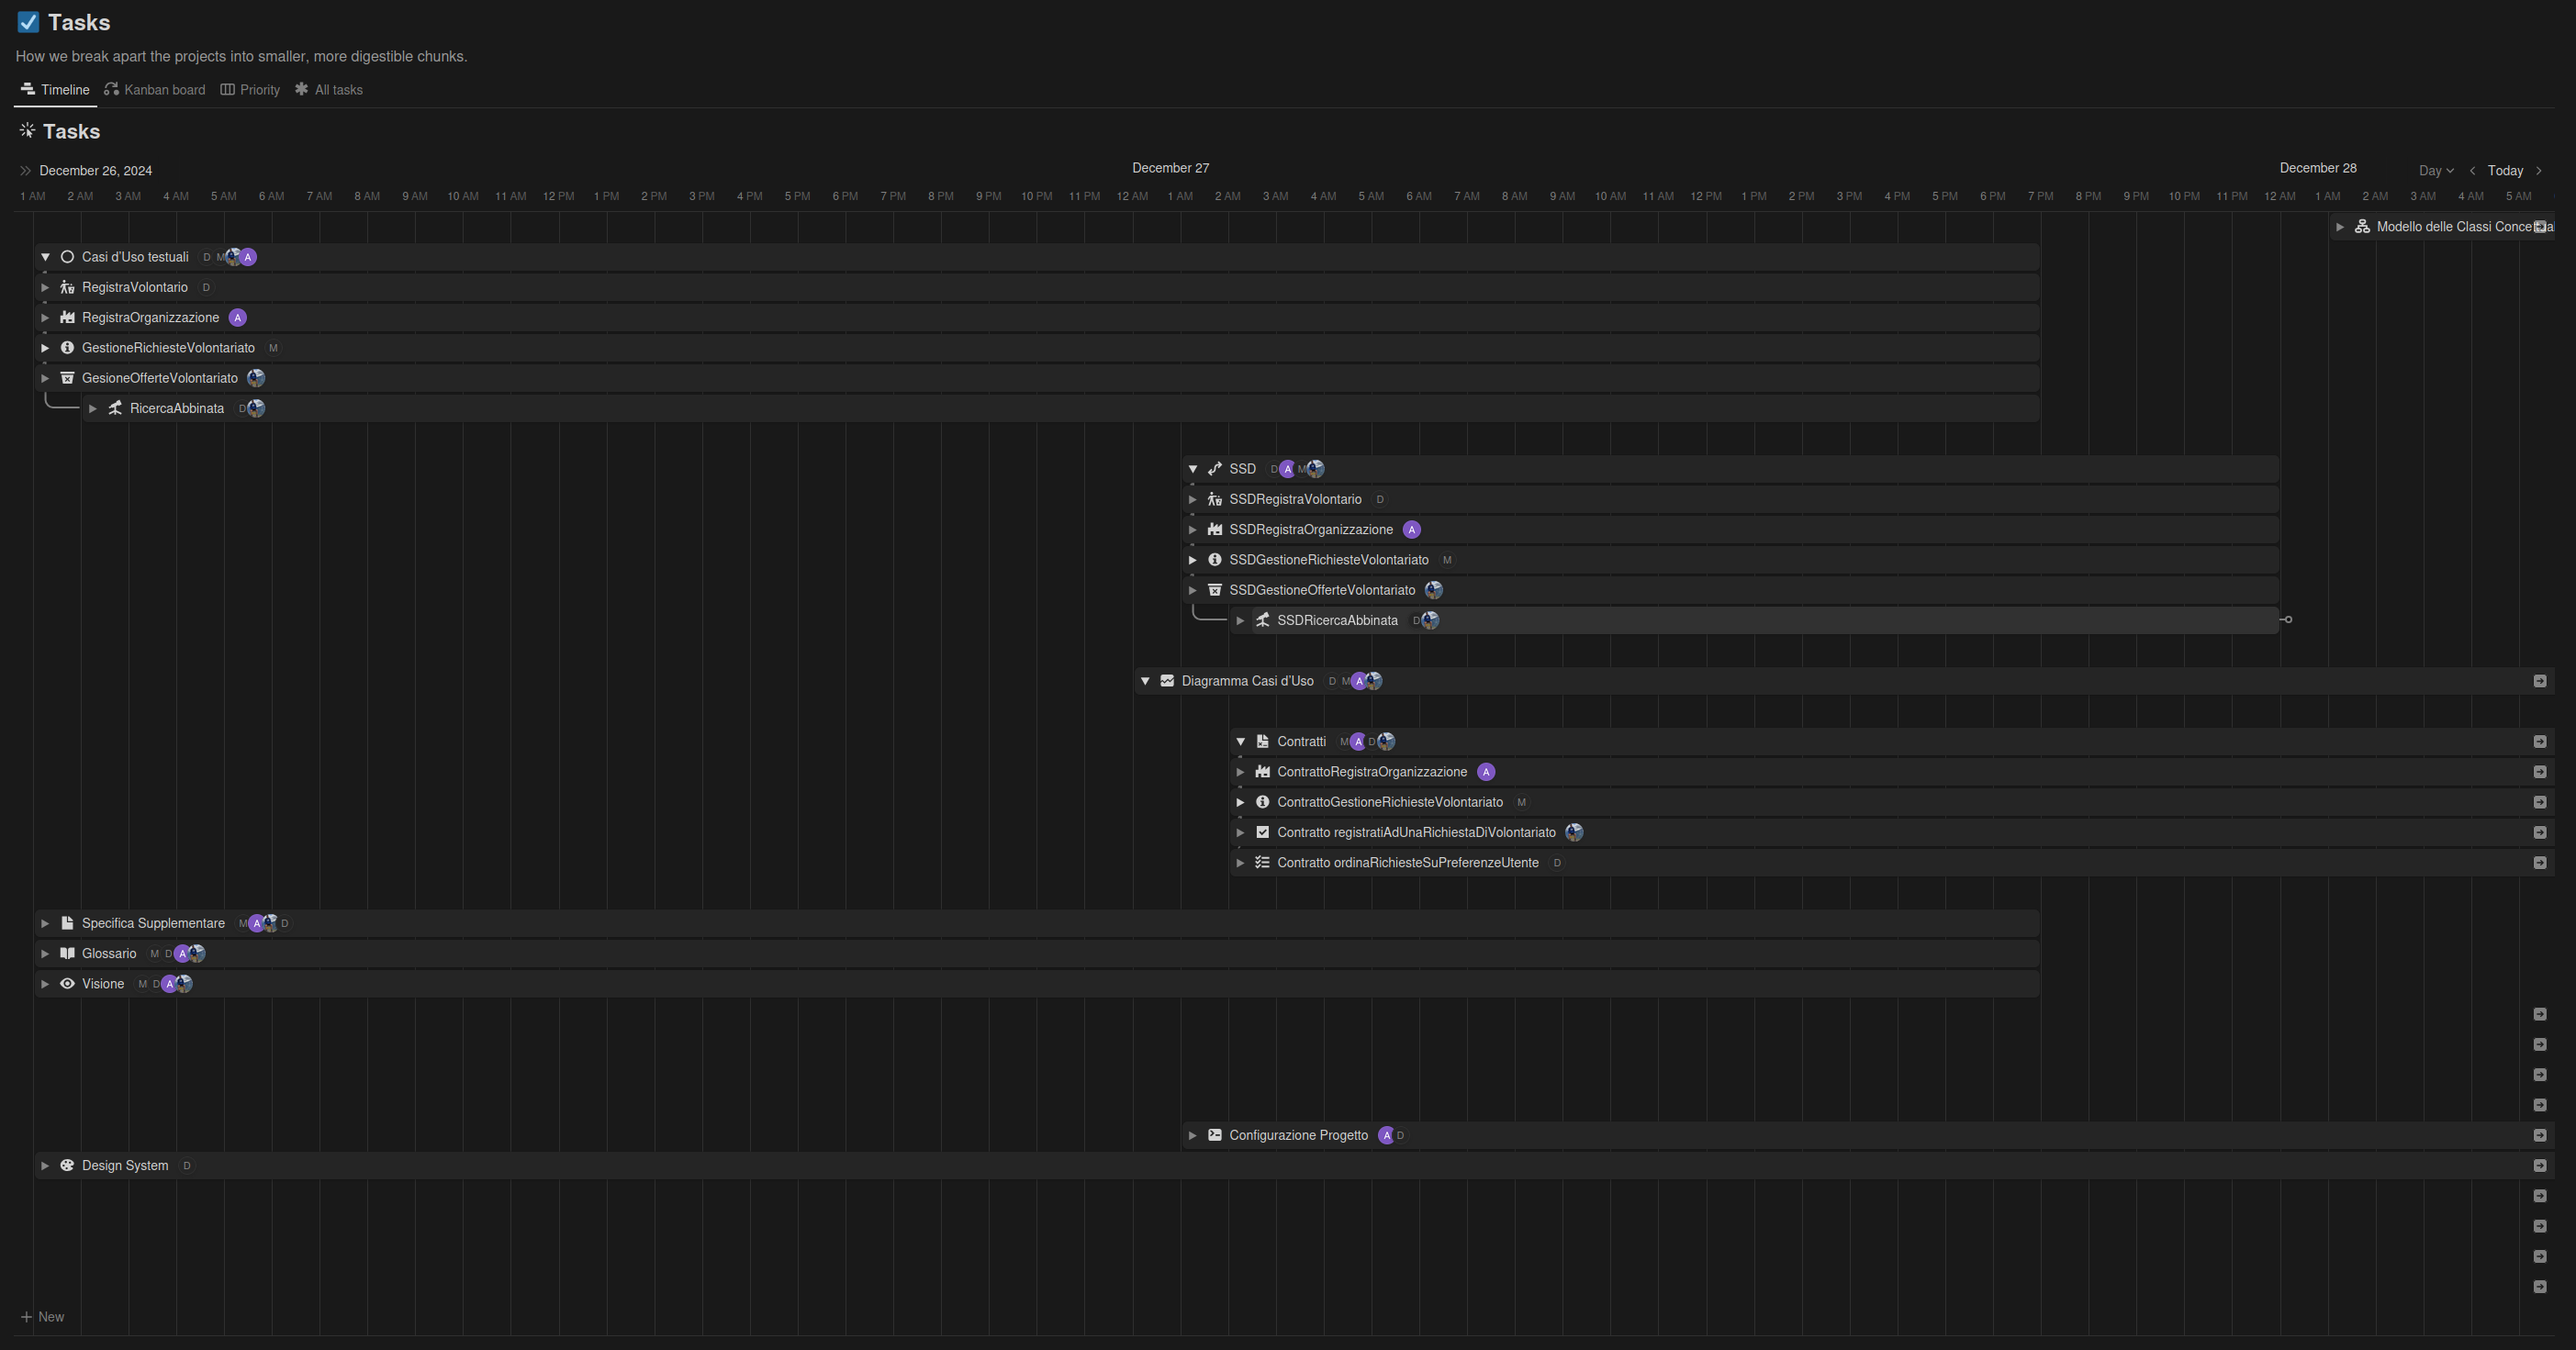
\includegraphics[width=\textwidth]{gantt-1}
        \caption{Diagramma Gantt del progetto DoIT - Parte 1}
        \label{fig:gantt1}
    \end{figure}

    \begin{figure}[h!]
        \centering
        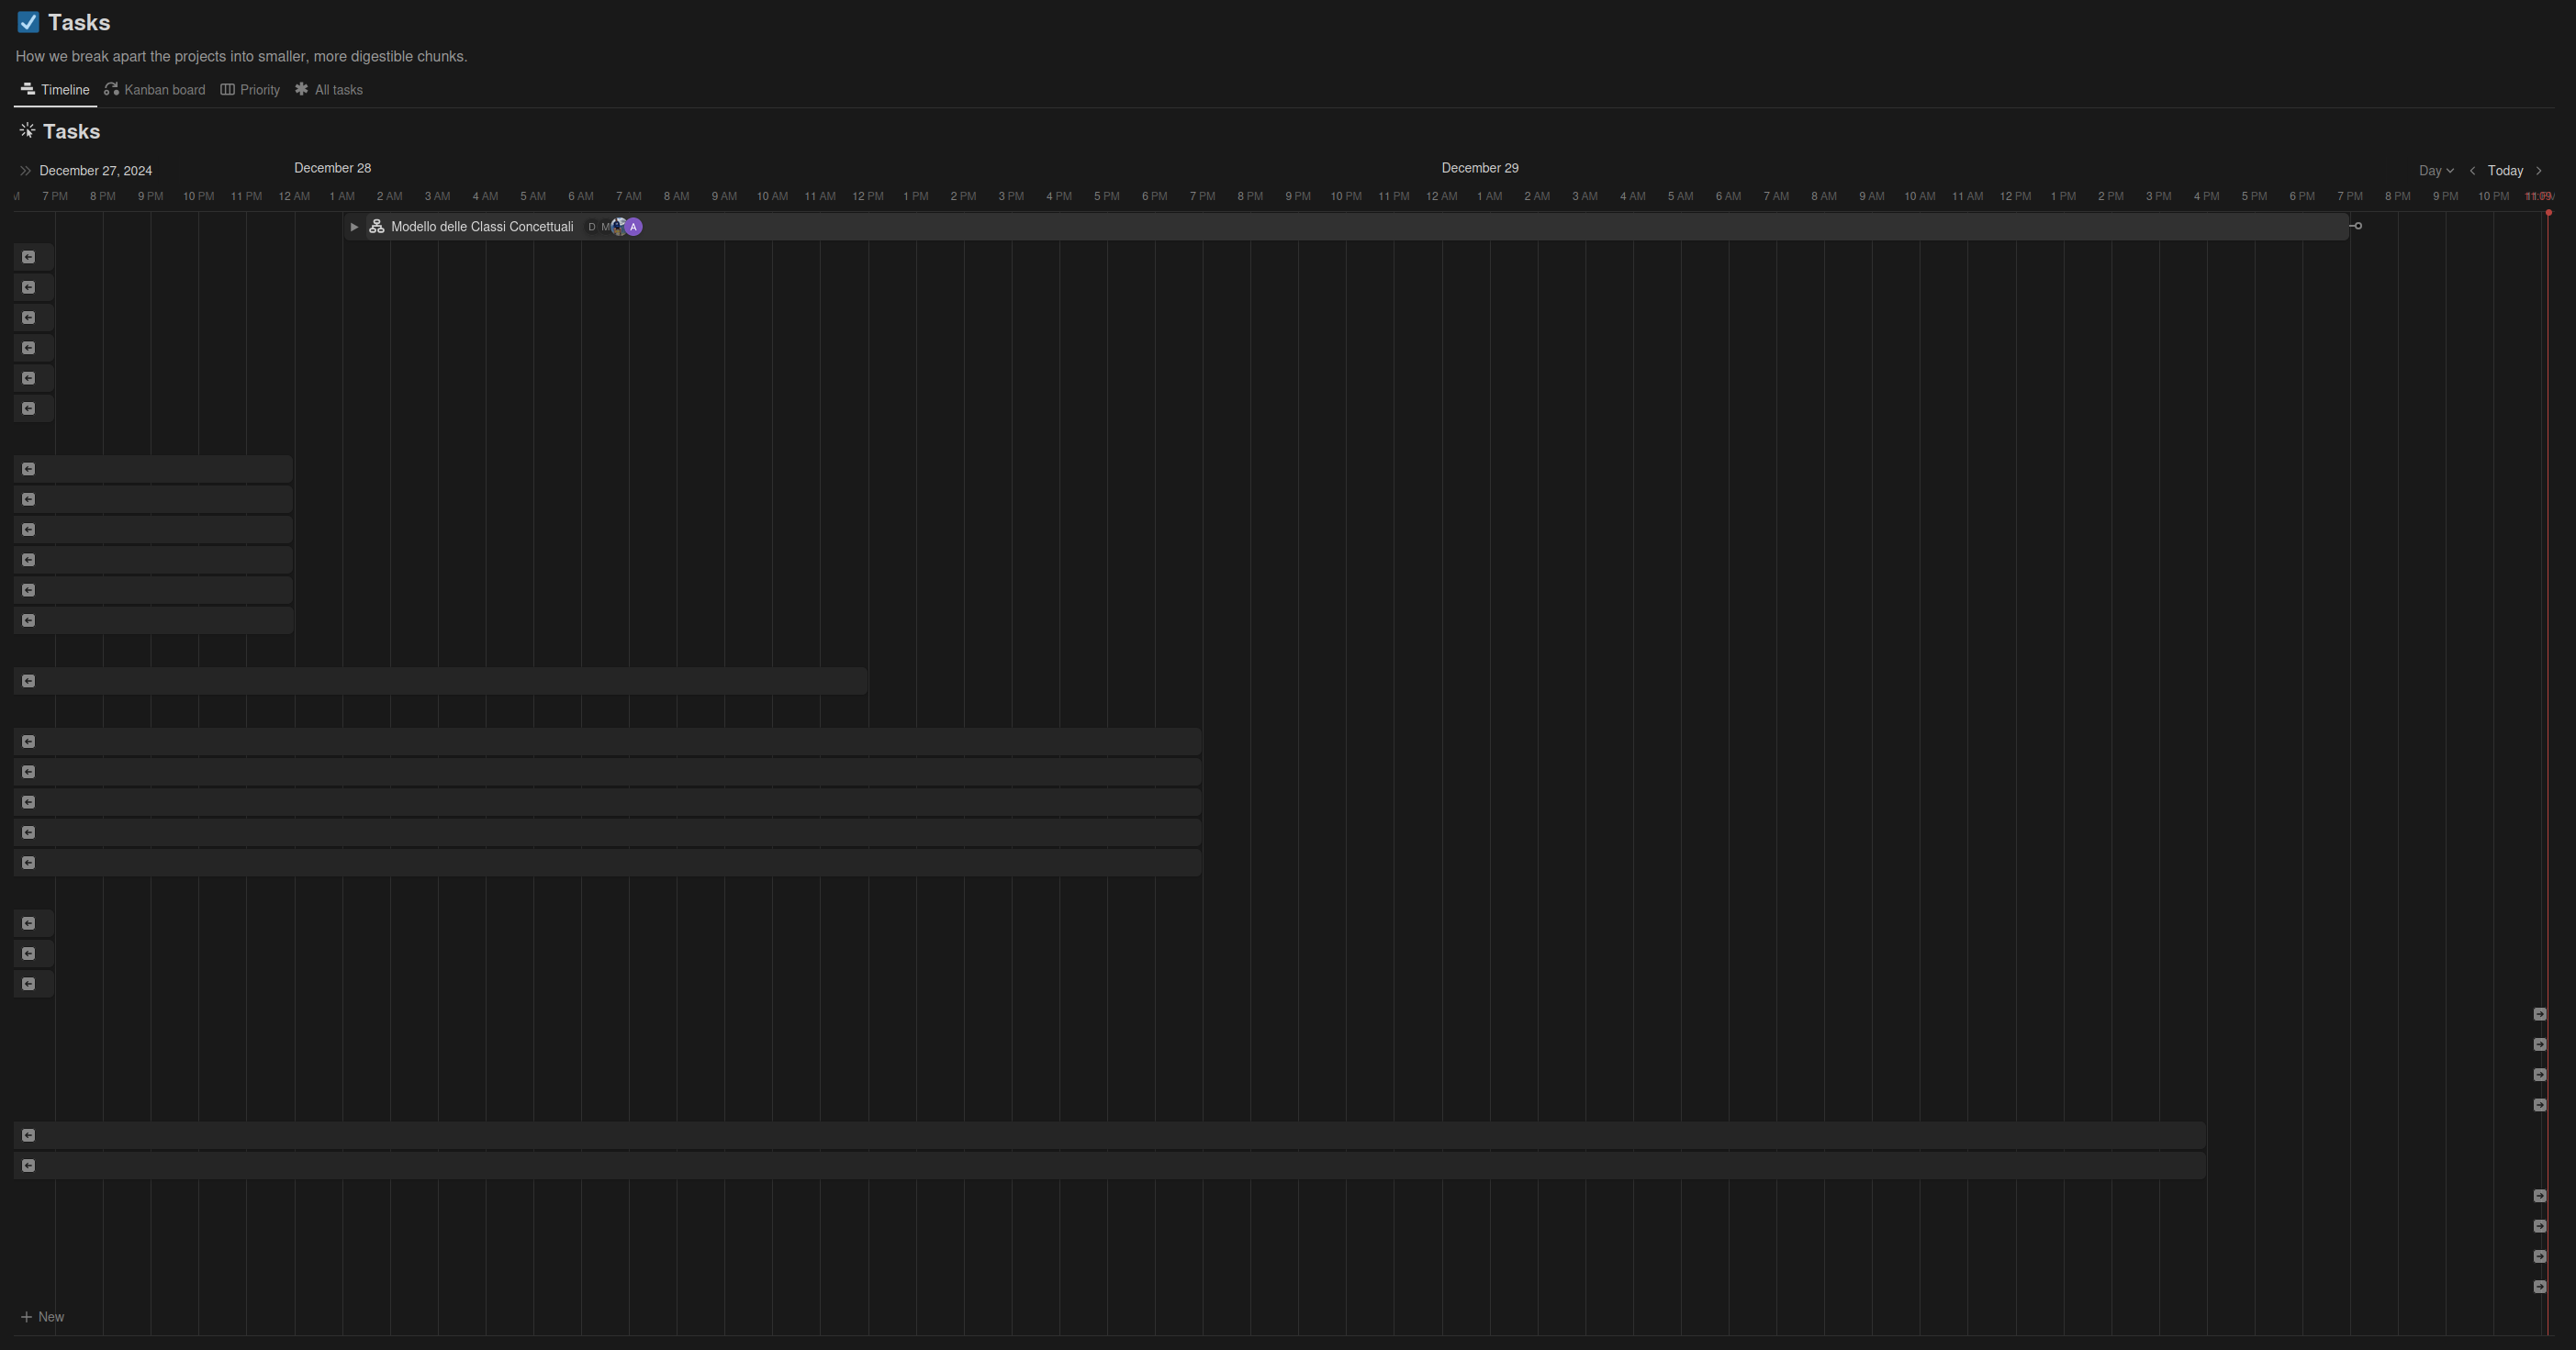
\includegraphics[width=\textwidth]{gantt-2}
        \caption{Diagramma Gantt del progetto DoIT - Parte 2}
        \label{fig:gantt2}
    \end{figure}

    \begin{figure}[h!]
        \centering
        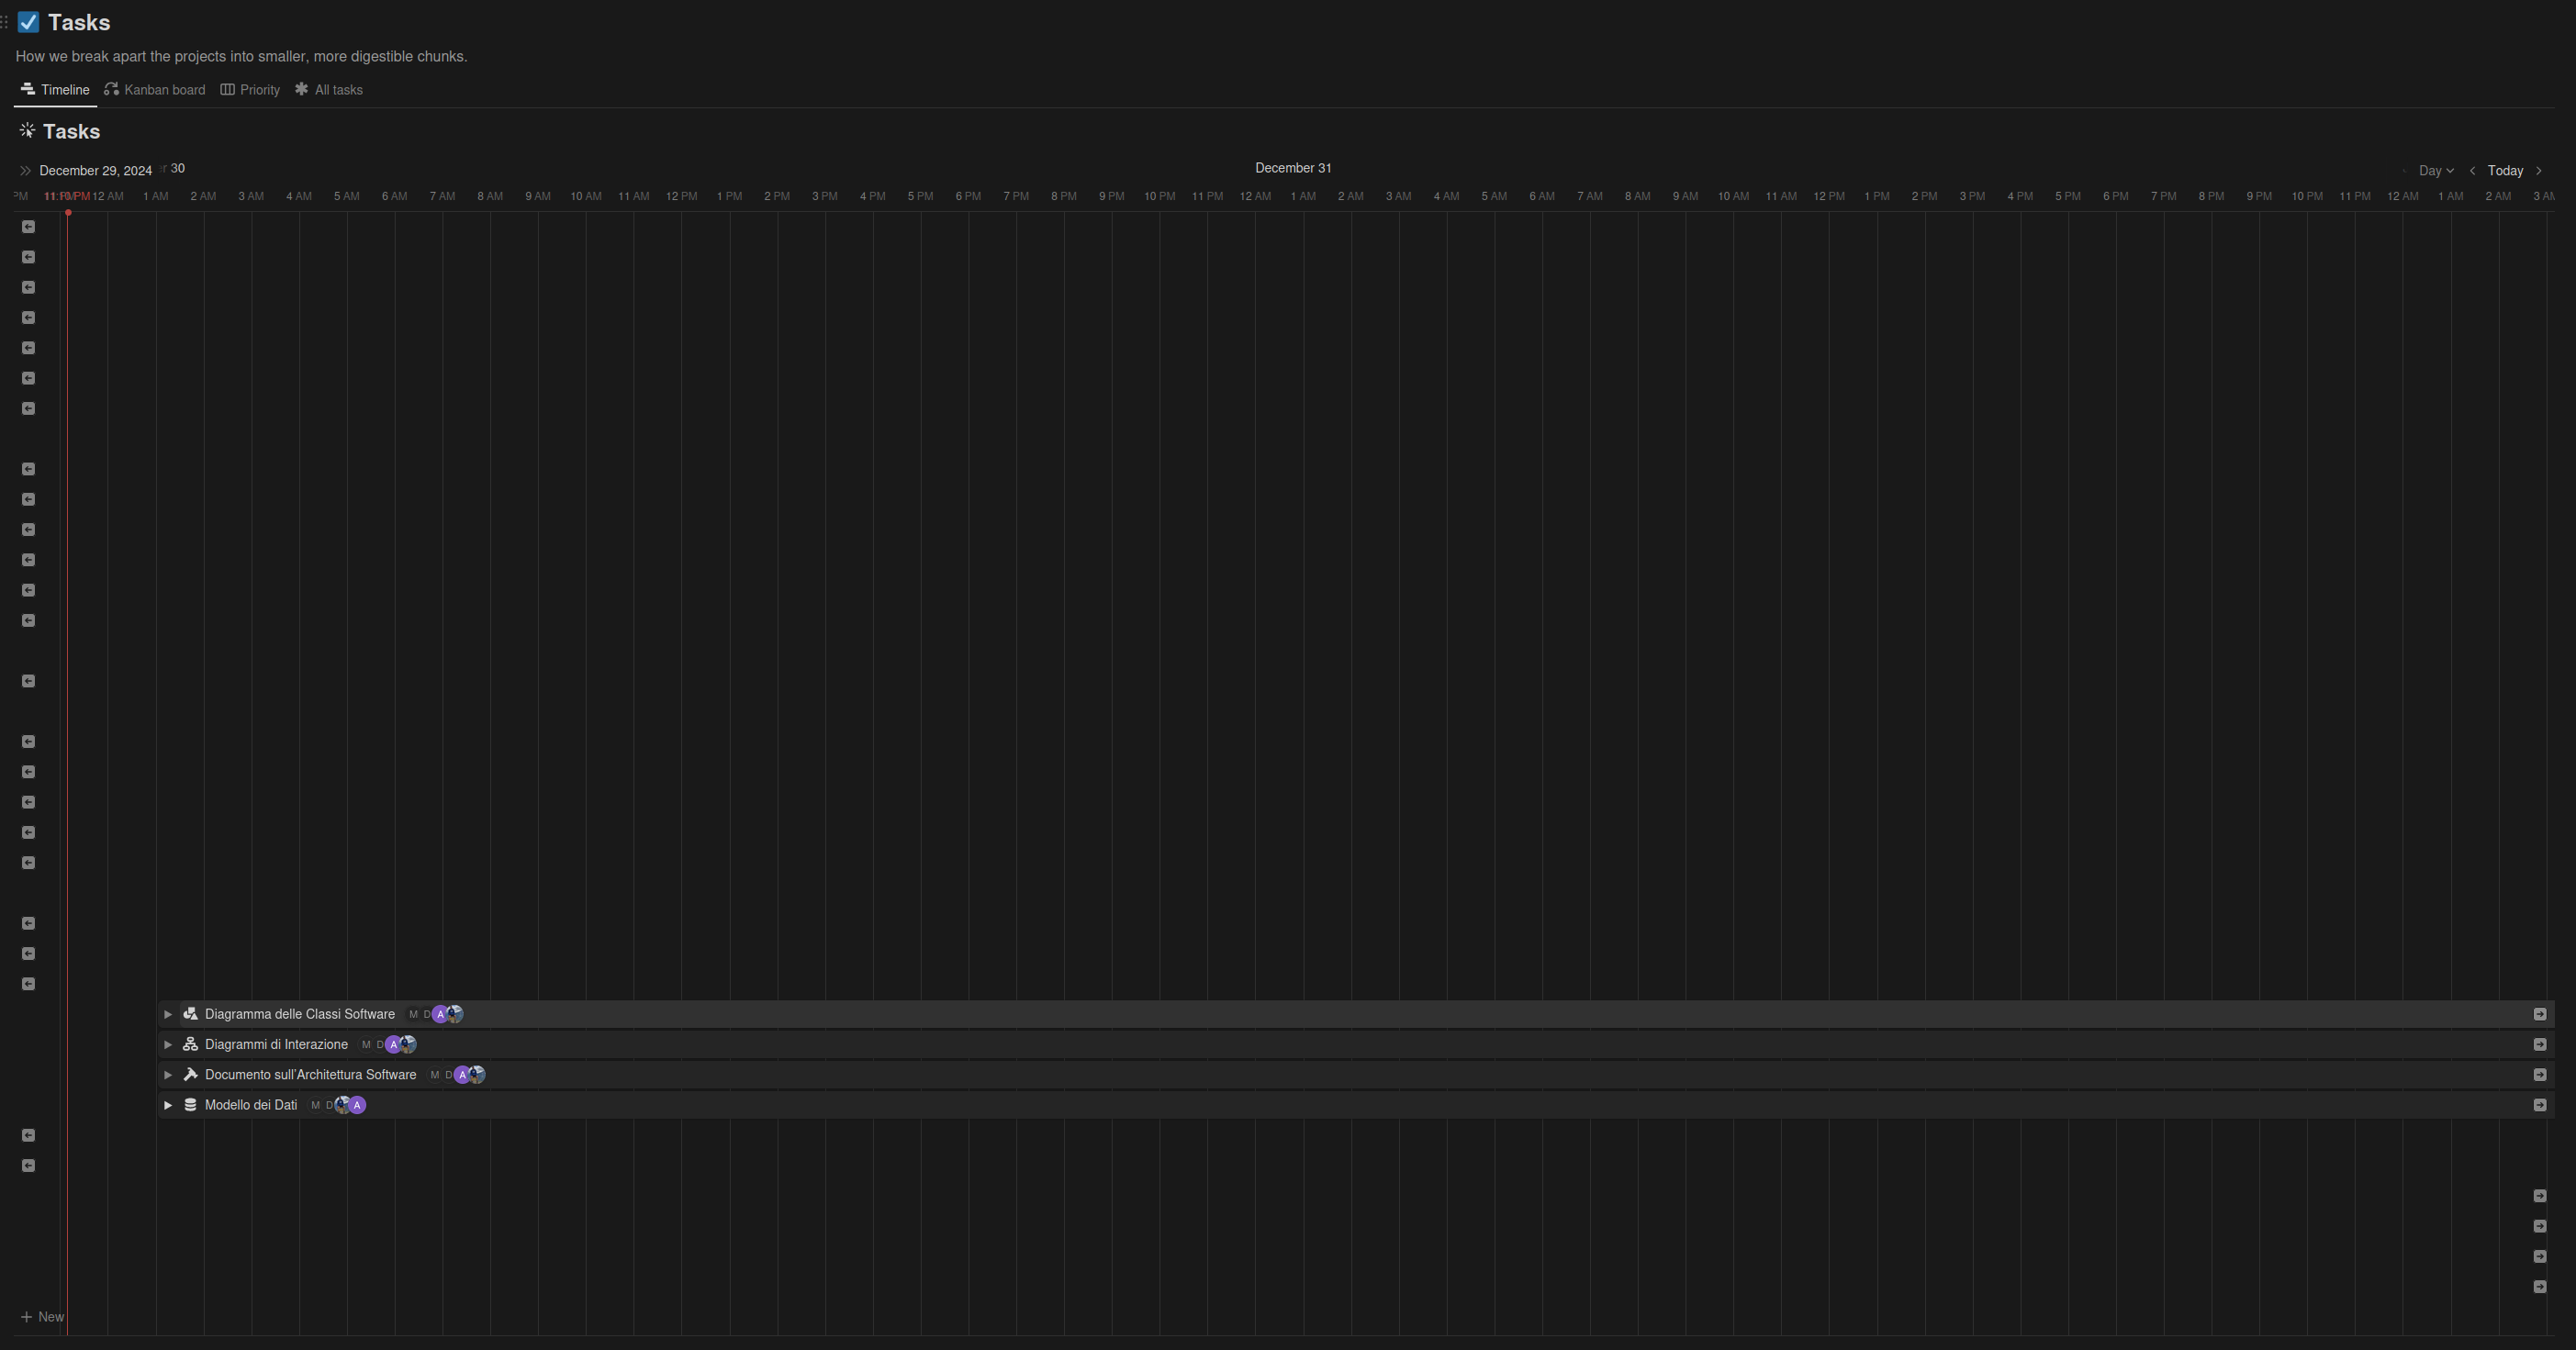
\includegraphics[width=\textwidth]{gantt-3}
        \caption{Diagramma Gantt del progetto DoIT - Parte 3}
        \label{fig:gantt3}
    \end{figure}

    \begin{figure}[h!]
        \centering
        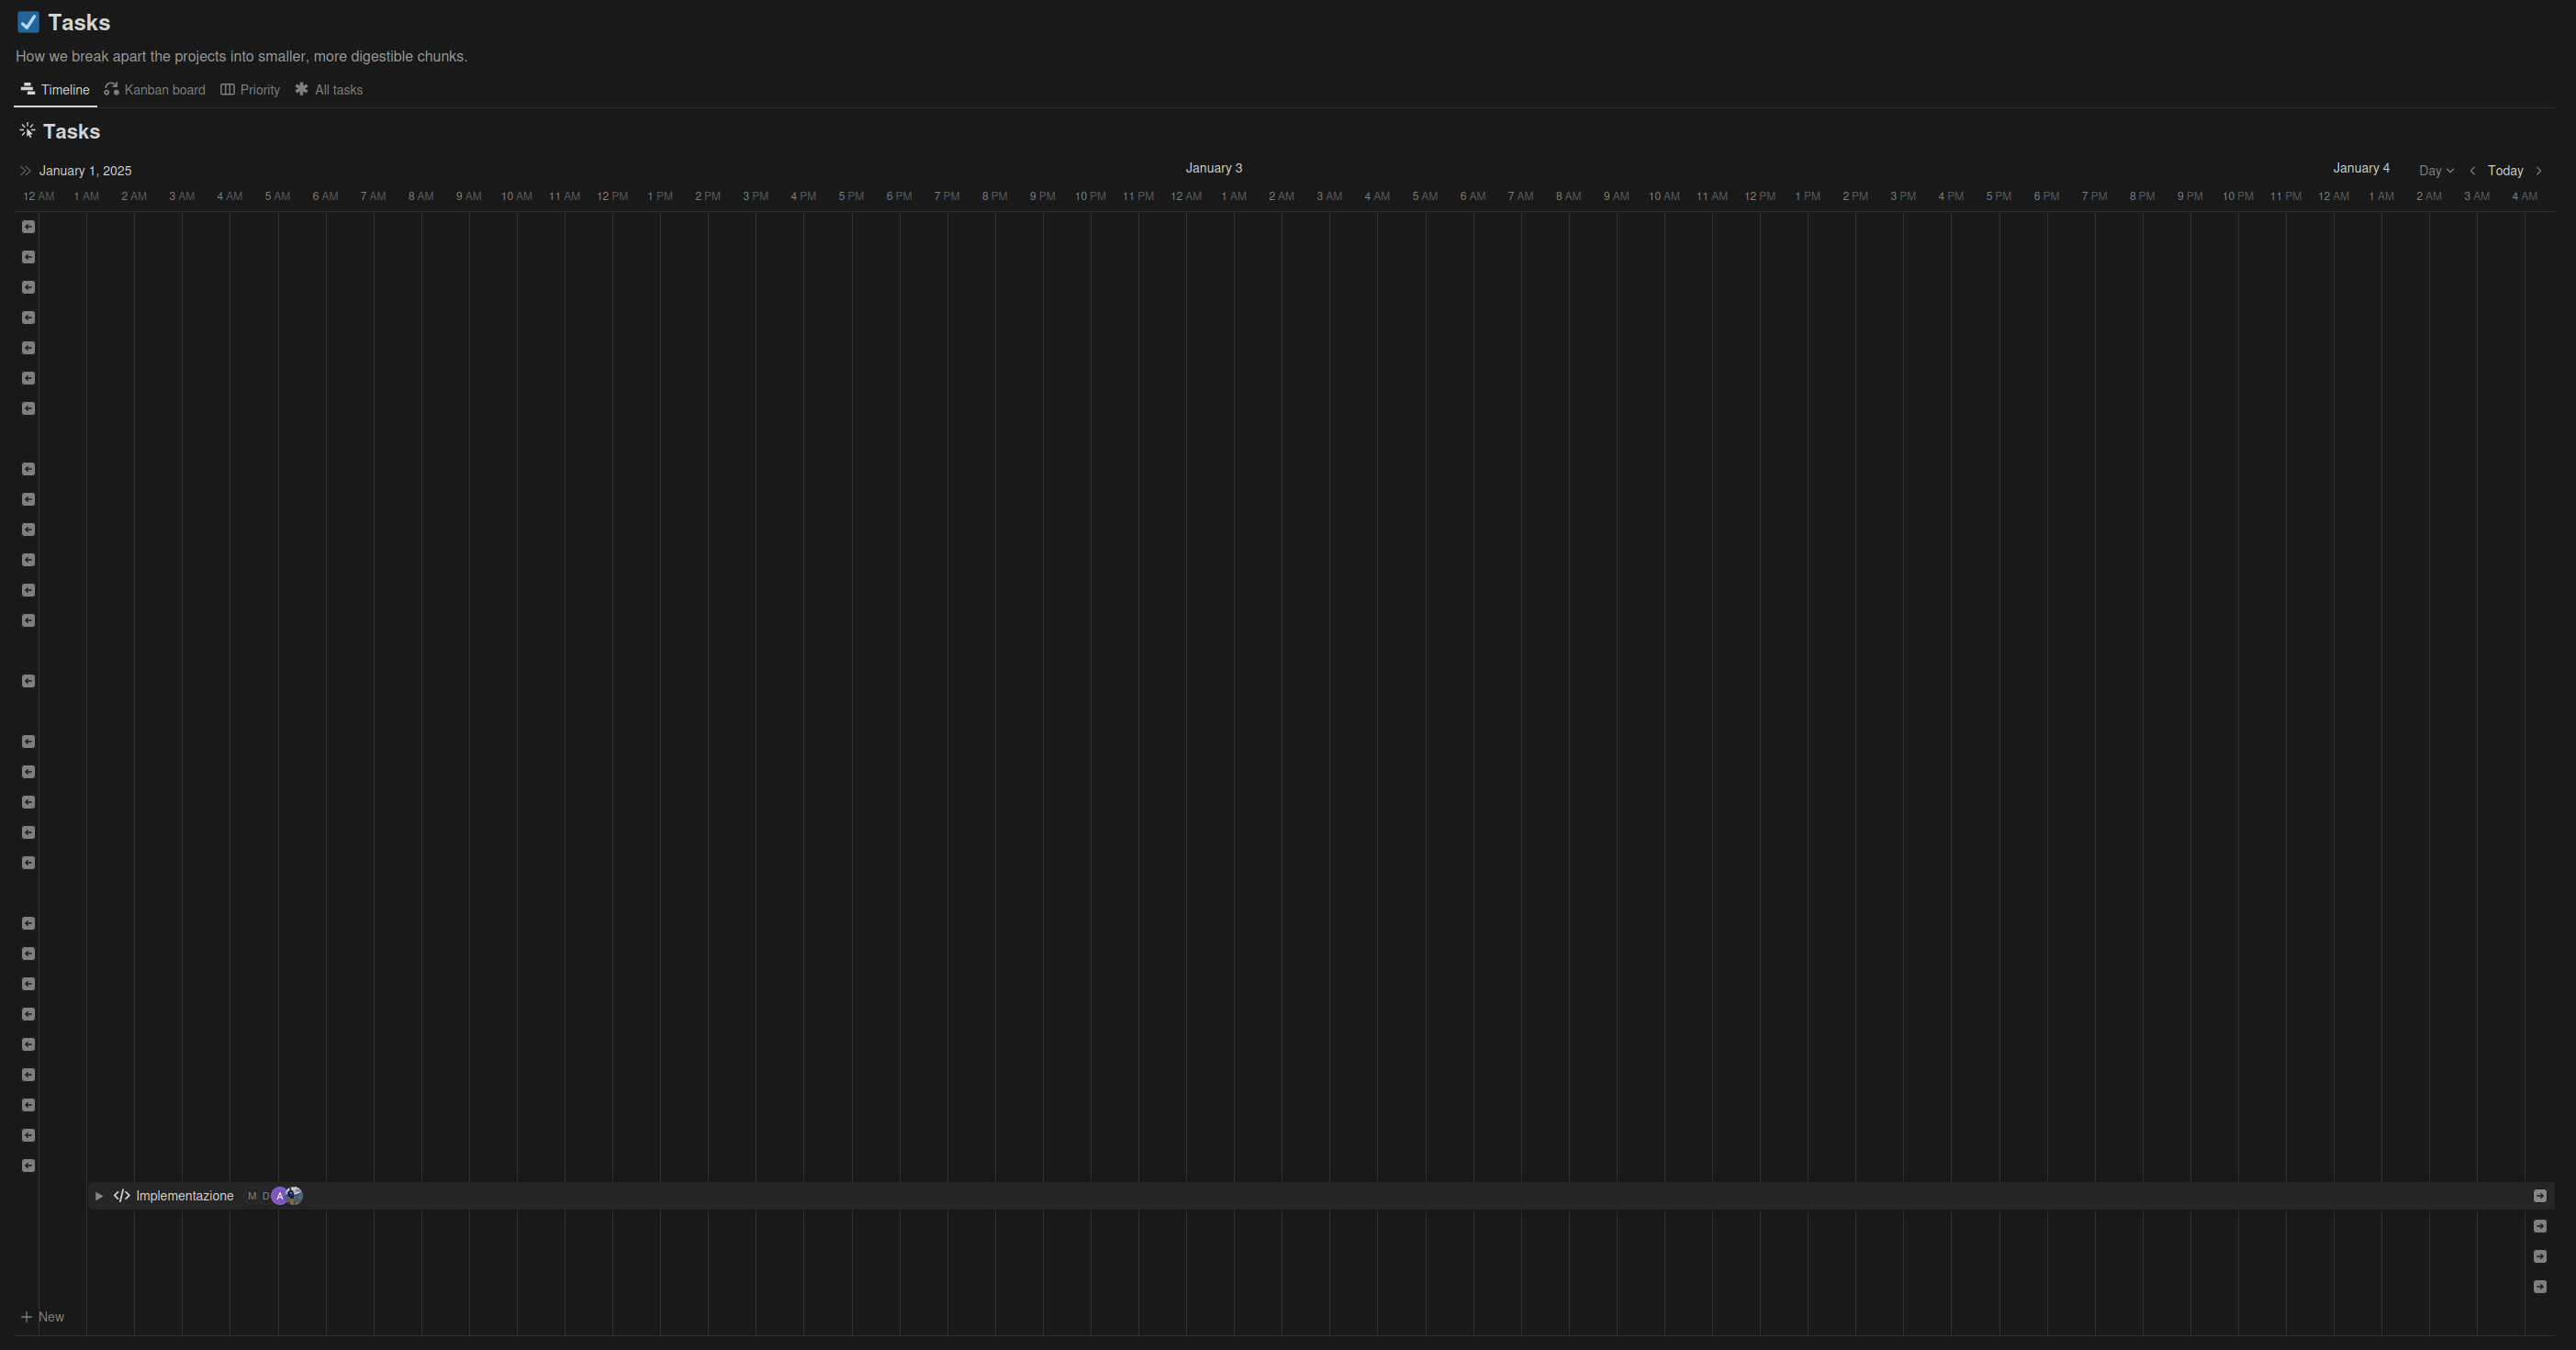
\includegraphics[width=\textwidth]{gantt-4}
        \caption{Diagramma Gantt del progetto DoIT - Parte 4}
        \label{fig:gantt4}
    \end{figure}

    \begin{figure}[h!]
        \centering
        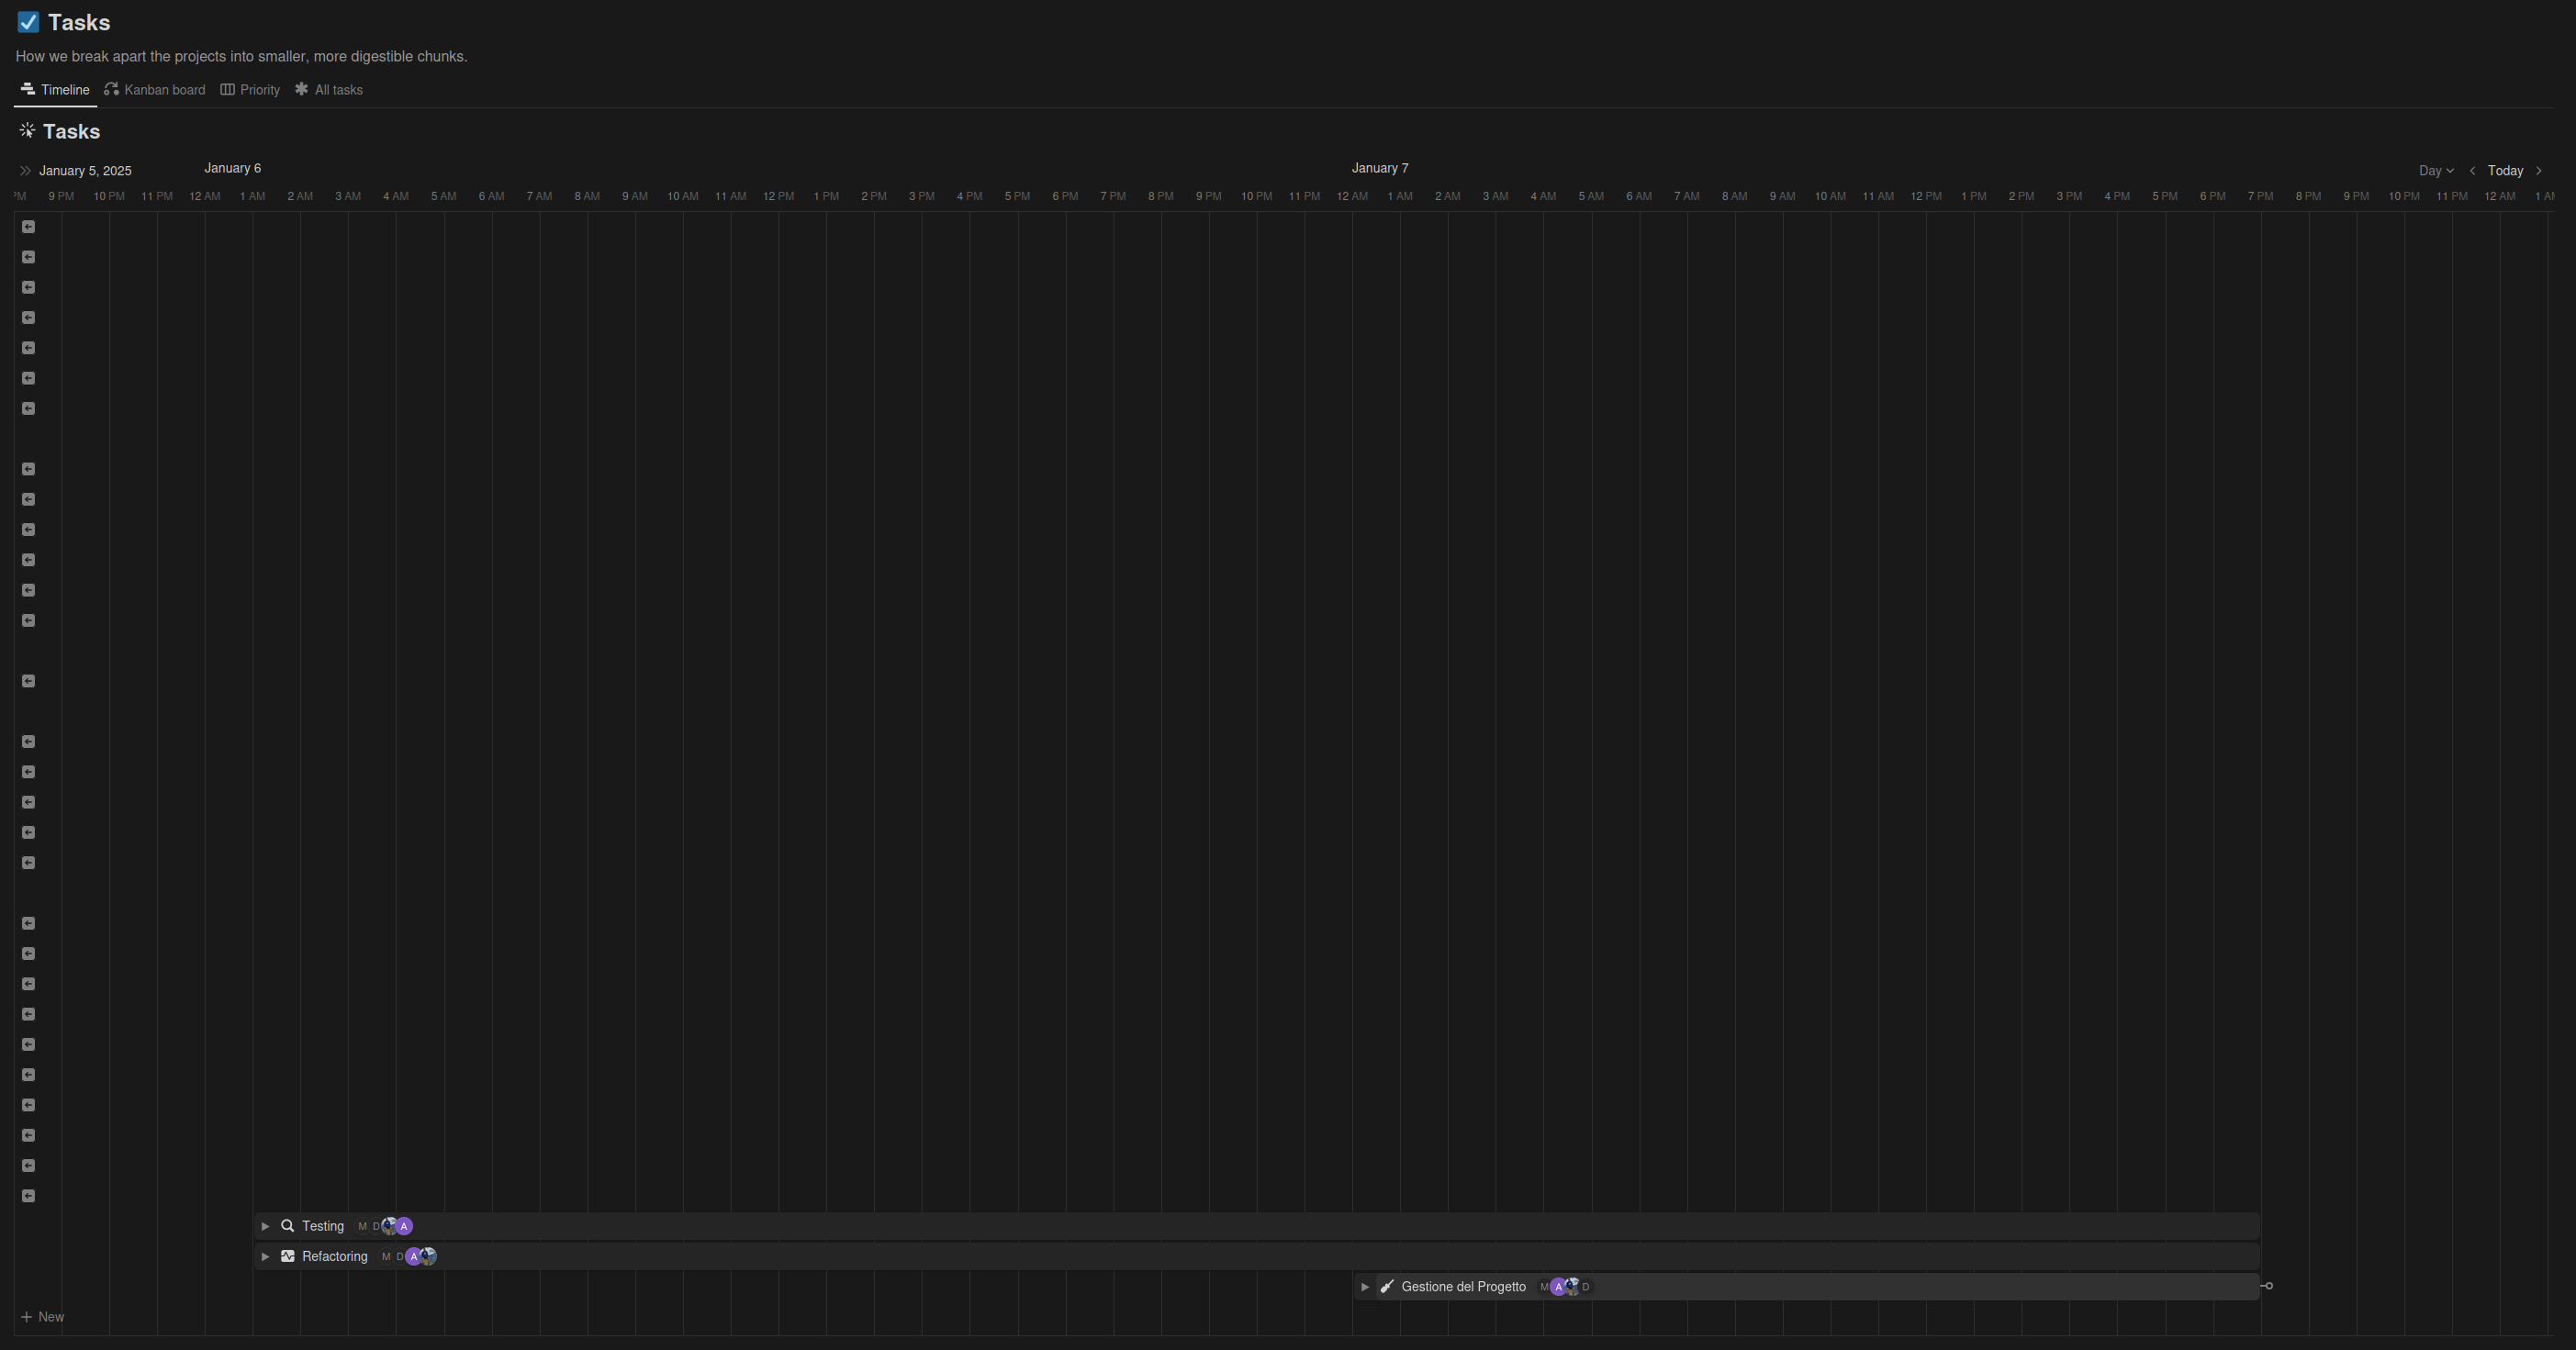
\includegraphics[width=\textwidth]{gantt-5}
        \caption{Diagramma Gantt del progetto DoIT - Parte 5}
        \label{fig:gantt5}
    \end{figure}

    \newpage

    \chapter{Requisiti}\label{ch:requisiti}
% Your content here

    \newpage

    \chapter{Iterazione 1: Requisiti}\label{ch:iterazione-1:-requisiti}
% Your content here

\end{document}